\begin{figure}[htbp]
  \centering
    \begin{subfigure}[b]{0.45\textwidth}
    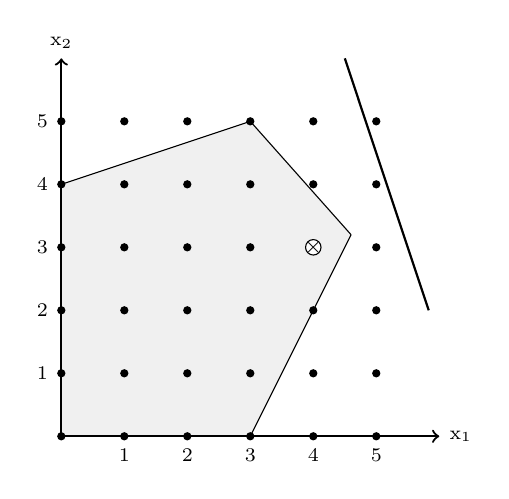
\begin{tikzpicture}[scale=0.8,font=\scriptsize]
      \centering
      \fill[fill={rgb:black,1;white,16}] (0,0) -- (0,4) -- (3,5) -- (4.6,3.2) -- (3,0) -- cycle;
      \draw [<->,thick] (0,6) node (yaxis) [above] {\sansitalicfont
      x\textsubscript{2}}
        |- (6,0) node (xaxis) [right] {\sansitalicfont x\textsubscript{1}};

      \foreach \x in {1,...,5} \node at (\x,-0.3) {\sansfont \x};
      \foreach \y in {1,...,5} \node at (-0.3, \y) {\sansfont \y};

      \draw (0, 4) -- (3,5);
      \draw (3, 0) -- (4.6,3.2);
      \draw (3, 5) -- (4.6,3.2);
      \draw [thick] (4.5,6) -- (5.833,2); 

      \foreach \x in {0,...,5} \foreach \y in {0,...,5}
        \draw (\x, \y) node[circle,fill=black, inner sep=0pt, minimum width=3pt,
        radius=2.5pt] {};
     
      \draw (4,3) node[circle,fill=white, inner sep=-0.9pt, draw=black, line 
      width=0.4pt] {\scriptsize$\times$};
    \end{tikzpicture}
      \caption{at the root node}
\label{fig:mipplot1}
    \end{subfigure}
  \begin{subfigure}[b]{0.45\textwidth}
    \centering
    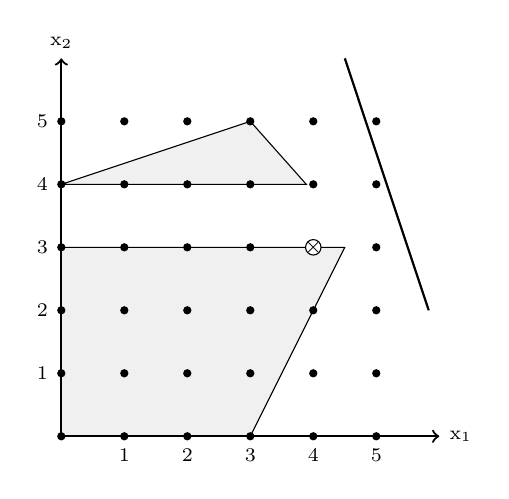
\begin{tikzpicture}[scale=0.8,font=\scriptsize]

      \fill[fill={rgb:black,1;white,16}] (0,0) -- (0,3) -- (4.5,3) -- (3,0) --cycle;
      \fill[fill={rgb:black,1;white,16}] (0,4) -- (3,5) -- (3.88889,4) -- cycle;

      \draw [<->,thick] (0,6) node (yaxis) [above] {\sansitalicfont
      x\textsubscript{2}}
        |- (6,0) node (xaxis) [right] {\sansitalicfont x\textsubscript{1}};

      \foreach \x in {1,...,5} \node at (\x,-0.3) {\sansfont \x};
      \foreach \y in {1,...,5} \node at (-0.3, \y) {\sansfont \y};
      
      % lower MIP
      \draw (3, 0) -- (4.5,3) -- (0,3);

      % upper MIP
      \draw (3.88889,4)--(0,4)--(3,5)--cycle;
      \draw [thick] (4.5,6) -- (5.833,2); 

      \foreach \x in {0,...,5} \foreach \y in {0,...,5}
        \draw (\x, \y) node[circle,fill=black, inner sep=0pt, minimum width=3pt,
        radius=2.5pt] {};
     
      \draw (4,3) node[circle,fill=white, inner sep=-0.9pt, draw=black, line 
      width=0.4pt] {\scriptsize$\times$};
    \end{tikzpicture}
    \caption{before first branching}
    \label{fig:mipplot2}
  \end{subfigure}
 \caption{Graphical representation of a typical MIP problem}
 \end{figure}
